\section{Solution}
\label{sec:Solution}

In order to pursue the goal of introducing contracts to BDD and easing the continued work on a given software development project, we introduce the Salad Framework. Salad contains three DSLs --- each with a specific purpose. Gherkin is the BDD feature specification language, Lettuce is the transformation language and lastly, Tomato is a simplified version of JML.  Combined, they make it possible for contracts to be extracted and generated from feature descriptions and transformed into JML. Figure \ref{fig:saladoverview} presents the workflow from input to output.

\begin{figure}
  \begin{center}
    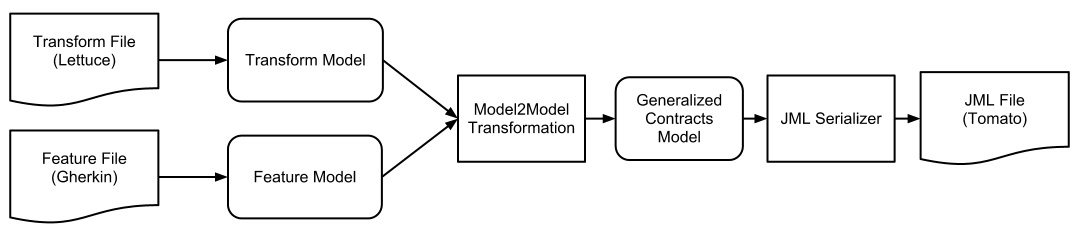
\includegraphics[scale=0.35]{images/framework_overview.png}
  \end{center}
  \caption{Salad Framework Overview}
  \label{fig:saladoverview}
\end{figure}

The Feature Model represents an extension of the feature language.
We want to allow people already familiar with BDD-features to work in an environment that they are accustomed to. 
This is achieved by extending the original, well-known feature language. 
We want the extending parts of the feature language we introduce in this project to be done with as much respect to the original feature language's textual syntax as possible. 
Having this rich model and language, that contains both the original features of the feature language as well as our extension, 
also allows for further development on the project as all elements of the language are available in the model. 
One could do a transformation to a simplified model accepted by standard BDD tools, which will allow the further generation of regular test-cases.

Lettuce specifies how the contracts written in natural language in the feature file are transformed to actual contracts.
By specifying rules on how contracts are interpreted, the user decides the nature of the language in which the natural language contracts are represented. 

Through model-to-model transformation, the feature model(s) and the transform model(s) are transformed into a generalized model representing contracts describing the pre- and postconditions. The textual representation of our JML model resembles Java syntax with classes containing methods and their contracts written in JML. 

\subsection{A Generalized Model for Contracted Software}
\label{sub:AGeneralizedModelforContractedSoftware}

In order to make our framework modularized and support multiple output programming languages, we have designed a generalized model which
we can make transformations to (see Figure~\ref{fig:generaloutputmodel}).

\begin{figure}
  \begin{center}
    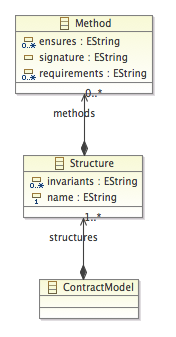
\includegraphics[scale=0.35]{images/generalized_outputmodel.png}
  \end{center}
  \caption{A General Model for Representing Contracted Software Systems}
  \label{fig:generaloutputmodel}
\end{figure}

The model consists of a number of structures, e.g. classes or interfaces, that contain a number of methods.
In the model we support the most common contracting features, namely preconditions, postconditions and invariants.
This allows definition of independent target languages based on the model for serialization, such as in our case Tomato for JML(\ref{sub:Tomato-aJML-compatibleLanguagefortheGeneralizedContractedSoftwareModel}).

% Insert sentences about contracted model
